

\begin{figure*}[htb!]
	\centering
	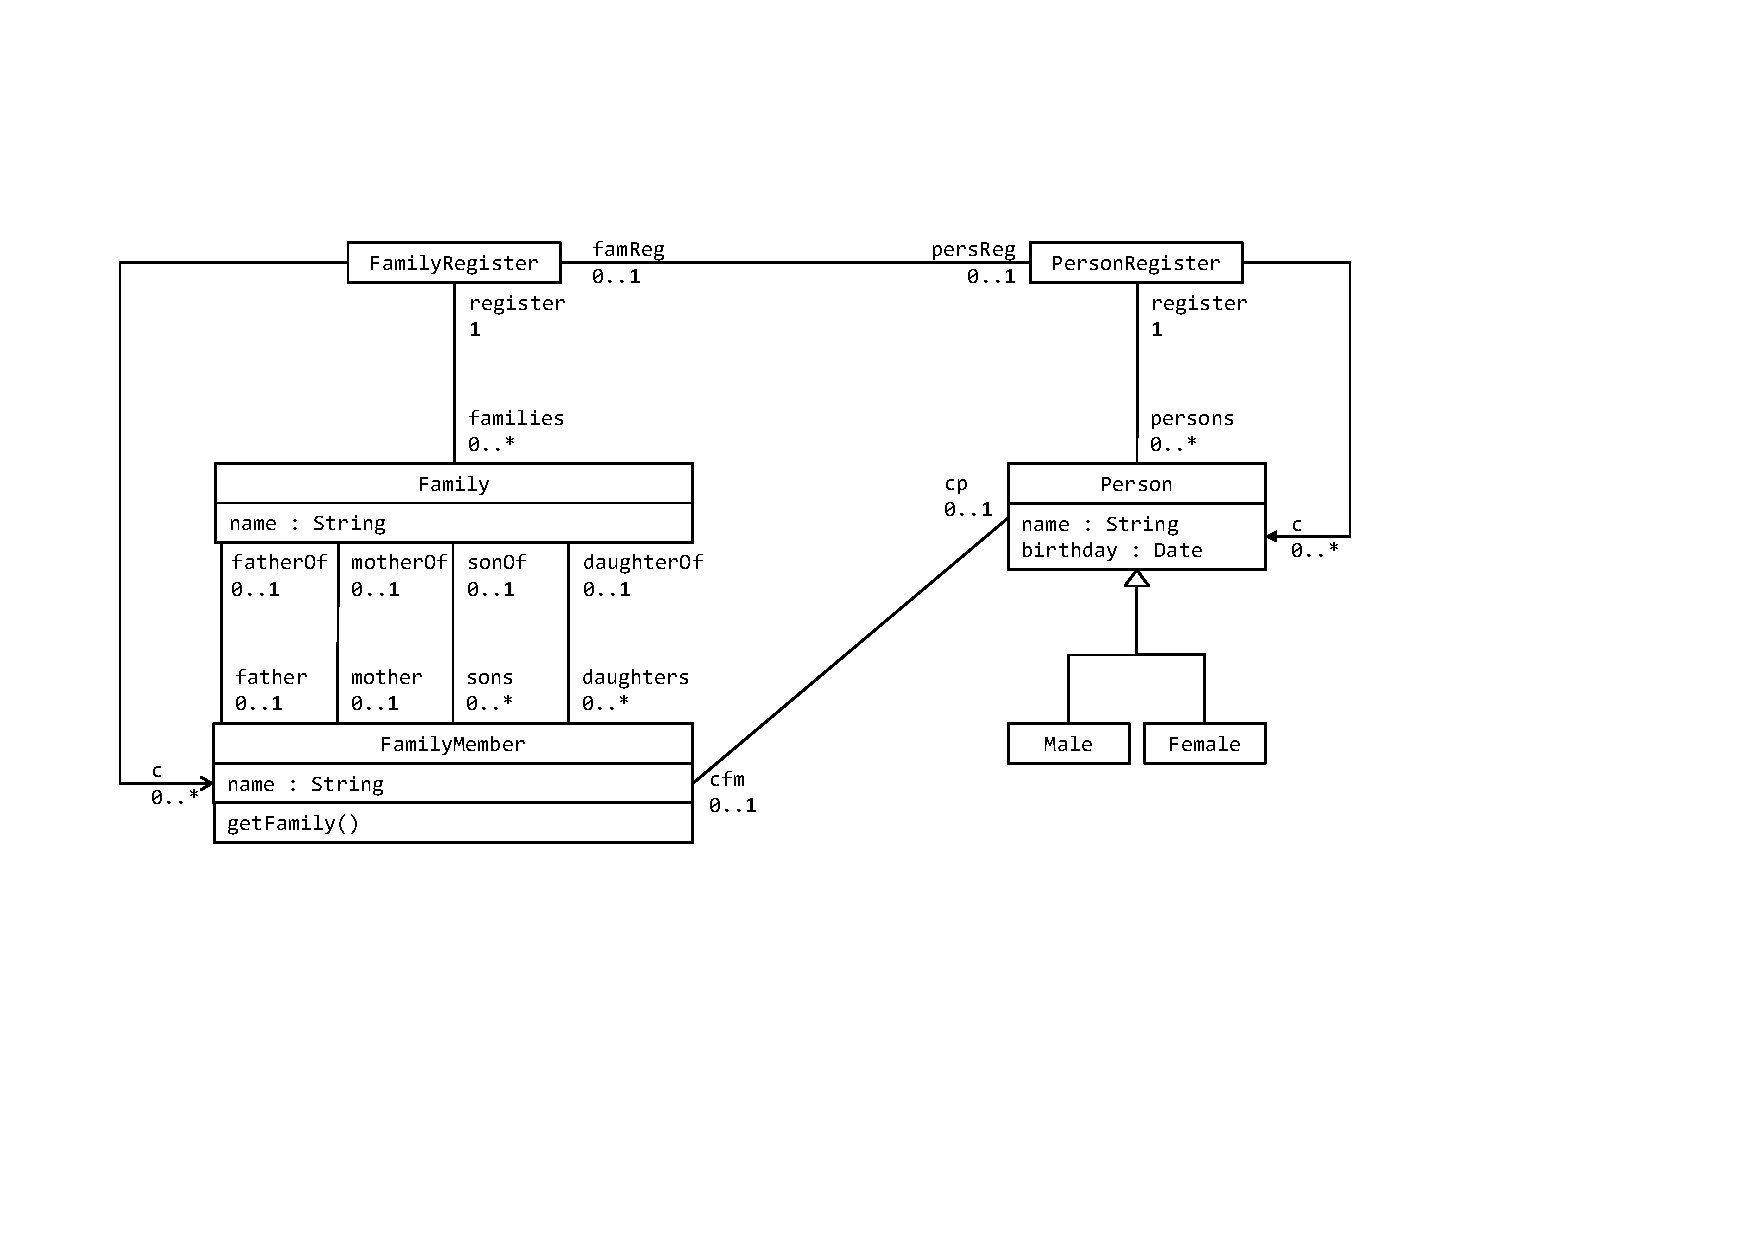
\includegraphics[width=0.75\textwidth]{diagrams/solutions/SDMLibModel}
	\caption{SDMLib model used for the benchmark}
	\label{fig:SDMLibModel}
\end{figure*}

\subsection{SDMLib}
\label{sec:SDMLib}

\NOTE{\emph{Solution expert:} Albert, \emph{Interviewer:} Thomas}

SDMLib, short for \emph{Story Driven Modeling Library}\footnote{http://www.sdmlib.org}, is a Java library to support Story Driven Modeling \cite{Norbisrath2013}, a formalism based on graph transformations \cite{Ehrig2006}. In contrast to its predecessor Fujaba \cite{Nickel2000}, where model and story diagrams were specified using a graphical syntax, SDMLib purely relies on a textual syntax realized as an internal Java DSL. SDMLib is not a bx tool, but nevertheless it is included here as a model transformation tool against which bx tools may be compared. 

Model instances can be interpreted as \emph{graphs}, since a model typically constitutes a spanning containment-tree whose elements are interconnected with cross-tree edges. Consequently, model transformations can also be regarded as a problem in the domain of graph transformations. Graph-based systems can be classified into two different categories: Graph-rewrite systems and graph grammars, which constitute the foundation of SDMLib and eMoflon, respectively. 

\emph{Graph rewriting} means that graphs are transformed by applying graph rewrite rules. A graph rewrite rule specifies the replacement of a graph pattern (left-hand side) by a subgraph to be embedded into the overall host graph. Graph rewrite rules may be used to specify in-place model transformations. However, they may also be employed for model-to-model transformations by applying them to multiple graphs. In case of bidirectional and incremental transformations, both directions as well as the incremental mode of operation need to be specified explicitly. The solution in SDMLib demonstrates this approach.

\subsubsection{Classification}
SDMLib's architectural style is \emph{restoration-based}, following \emph{initial-diag-based} application scenarios (table \ref{tab:features-all-tools}). The left part of figure \ref{fig:initialDiagBased} depicts the restoration-based architecture for initial-diag-based scenarios, where the transformation programmer takes a diag and needs to specify the manipulation of the dependent model until both models are consistent again. 

No formal guarantees are provided by SDMLib: both synchronization directions are specified separately and independently. As a consequence, the transformation developer needs to ensure, that both directions actually match in a bidirectional synchronization. Analogously to the BXtend solution this can be viewed as an advantage, since the bx programmer may freely decide whatever is necessary to solve the current task.

In SDMLib, there is no explicit notion of \emph{consistency} as it is \emph{implicitly} given by the implemented pair of \emph{fCR/bCR}. Accordingly, synchronization \emph{control} is \emph{explicit}. Finally, SDMLib supports \emph{automatic} and \emph{directed} synchronization \emph{on demand}.

\subsubsection{Benchmark solution with SDMLib}
%The SDMLib solution of the benchmark is the only solution presented here, which needed modifications in the benchmark as it does not provide an adapter to transform the internal data structure to the respective EMF models and vice versa. While it would have been possible technically to provide an adapter which performs this task, the solution providers decided to modify the benchmark code instead. 



The following description is based on the SDMLib solution for the Families to Persons benchmark at TTC 2017 \cite{Zundorf2017}. Since SDMLib is designed for in-place transformations on a single host graph, the solution for the Families to Persons benchmark relies on a single graph which is created as internal data structure and comprises the contents of both models as well as explicit correspondence links between the respective elements. 

The respective \emph{graph metamodel} is depicted in figure \ref{fig:SDMLibModel}. To facilitate the comparison to the metamodels for the families and persons models depicted in figure~\ref{fig:metamodels}, we employ Ecore notation (without using containment conferences, which are not supported in SDMLib). To support incrementality efficiently, unidirectional references between \code{FamilyRegister} and \code{Fami\-lyMember} and \code{PersonRegister} and \code{Person} are added in order to detect changed elements. Finally, the correspondence model is represented with the help of links instantiated from two bidirectional references.


%In order to provide an impression of the benchmark solution with SDMLib, figure~\ref{fig:metamodels} depicts the graph metamodel that is created for both source and target model. Please note that it is a flat collection of model elements, where both source and target model elements of the transformation task are present in one single model without any containment hierarchy. In addition correspondence links between \code{FamilyRegister} and \code{PersonRegister} and between \code{FamilyMember} and \code{Person} are introduced. Furthermore, in order to support incrementality, unidirectional links between \code{FamilyRegister} and \code{FamilyMember} and \code{PersonRegister} and \code{Person} are added in order to detect changed elements.



\begin{lstlisting}[label={lst:sdmlib}, float=*t, language=java, caption={Forward transformation in SDMLib}]
private void transformForward() {
    familyRegisterPO = new FamilyRegisterPO().withPatternObjectName("fr");
    PersonRegisterPO personRegisterPO = familyRegisterPO.createPersonRegisterPO()
        .withPatternObjectName("pr");
    FamilyMemberPO memberPO = familyRegisterPO.createCPO().withPatternObjectName("fm");

    // there is an old corresponding person
    memberPO.startSubPattern();
    PersonPO oldPersonPO = memberPO.createCpPO().withName("oldP");
    oldPersonPO.createCondition(p -> ensureNameAndGender(p));
    memberPO.endSubPattern();

    // no corresponding person
    memberPO.startNAC();
    memberPO.createCpPO().withPatternObjectName("noOldP");
    memberPO.endNAC();
    MalePO personPO = memberPO.createCpMalePO(Pattern.CREATE).withPatternObjectName("newP");
    personPO.createRegisterLink(personRegisterPO, Pattern.CREATE);
    personPO.createCondition(p -> ensureNameAndGender(p));
    
    familyRegisterPO.createLink(memberPO, Pattern.DESTROY);

    familyRegisterPO.rebind(familyRegister);
    familyRegisterPO.doAllMatches();	    
}
\end{lstlisting}

The core of the SDMLib solution consists of two graph rewrite rules, one for each direction. In Fujaba, the predecessor of SDMLib, graph rewrite rules were represented graphically as \emph{story patterns}; this notation was also used in the presentation of the SDMLib solution at TTC 2017 \cite{Zundorf2017}. Here, we stick to the actual textual notation instead, since the transformation developer operates on the source code level only\footnote{For presentation purposes, all metamodels are consistently given in graphical notation in this paper, regardless of the actual tool support.}.

Listing~\ref{lst:sdmlib} shows the graph rewrite rule for the forward transformation in SDMLib's internal DSL, embedded into Java. The internal DSL provides a programming interface for defining the elements of graph rewrite rules, as well as for launching their execution. The method for the graph rewrite rule uses code generated from the graph metamodel displayed in figure~\ref{fig:SDMLibModel}. 

The statements in line~2--4 define story pattern objects for the family register, the person register, and a family member, which need to be matched in the families model; the links connecting these objects are added implicitly to the story pattern by the called methods. 

Lines~8-11 handle the case that a corresponding person object already exists. This case is realized with an optional subpattern, which is started at line~8 and is terminated at line~11. The pattern is composed of an old person object which is connected to the family member object by a correspondence link. If pattern matching succeeds, the method \code{ensureNameAndGender} is called to restore consistency.

Lines~14--19 deal with the opposite case (there is no corresponding person object). To this end, a negative application condition is defined in lines~14--16. In lines~17--19, elements of story patterns are created which define the actions to be performed when the negative application condition holds: A person object has to be created and linked to the person register; then, the method \code{ensureNameAndGender} is called to establish consistency with the family object.

Finally, the temporary link between the family register and the family member --- which is set in the course of changes to the families model --- is matched and then removed (line~21), the story pattern object for the family register is bound (line~23), and the pattern is applied to all matches (line~24).   

 

%\begin{figure*}[tb!]
%	\centering
%	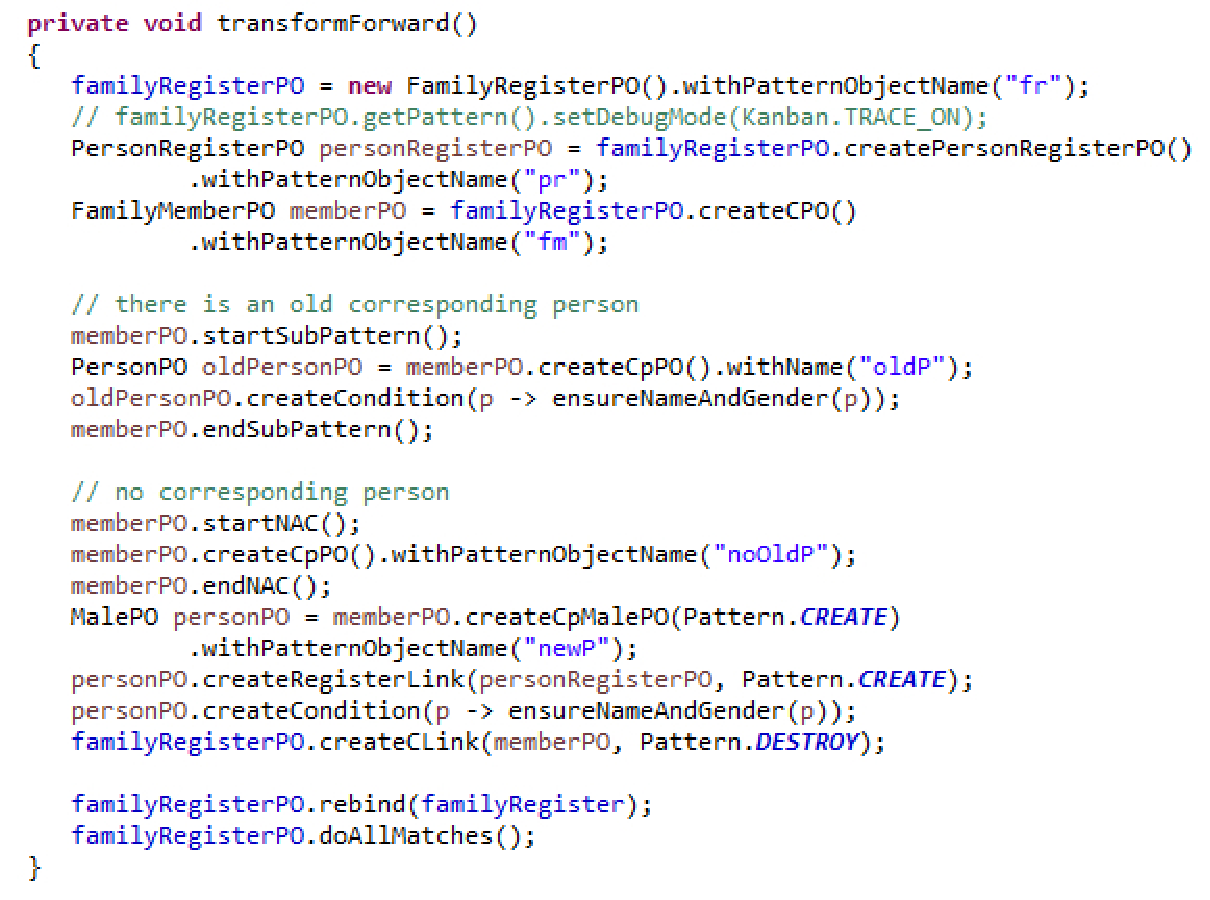
\includegraphics[width=0.75\textwidth]{diagrams/solutions/SDMLibForward}
%	\caption{Forward transformation in SDMLib}
%	\label{fig:SDMLibForward}
%\end{figure*}
%
%The Java code realizing the graph pattern for the forward transformation of the SDMLib solution is depicted in figure~\ref{fig:SDMLibForward}. The graph rewrite rule for the forward transformation is specified using code generated from the SDMLib data structure shown in figure \ref{fig:SDMLibModel}. It starts with establishing correspondence between the family and the person register. Afterwards, an optionally existing correspondence between the current family member and a previously transformed person is checked using the helper method \code{ensureNameAndGender()}. Then, the synchronization is specified using a negative application condition (NAC) enforcing that no person associated to the current family member already exists. In case the condition holds, a new person object is created and the correspondence link between the family member and the newly created person is established. Again the helper method \code{ensureNameAndGender} is used to create the proper person (male or female) and to compose the person's name. This graph rewrite rule is then bound to the actual \code{familyRegister} object and the matching engine is started to execute the rule. Please note that the transformation developer operates on the source code level only. However, for visualization purposes a graphical representation of the rule depicted above is given in the TTC paper describing the SDMLib solution \cite{Zundorf2017}.

